\lab{Algorithms}{B-Splines}{B-Splines}
Though B\'{e}zier curves are good for a variety of things, they have certain limitations.
\begin{itemize}
\item As the number of control points increases it becomes very expensive to compute the points on the curve.
\item Changes in the placement of a single control point affect the shape of the entire curve.
\item Since a change in any control point affects the entire curve, it is necessary to recompute the entire curve to account for any change in any control point.
\item As the number of points increases, individual points have progressively less affect on the portions of the curve that lie nearest to them.
\end{itemize}

B-Splines are an ideal way to answer these limitations.
A B-Spline is, roughly speaking, a piecewise B\'{e}zier curve.
In order to better explain what a Basis function is.

\section*{B-Spline Basis Functions}

In the previous lab we introduced a way to represent B\'{e}zier curves as a linear combination of Bernstein Polynomials.
Notice the convenient property that the coefficient of each Bernstein polynomial for the B\'{e}zier curve formed from a given control point is simply the control point itself.

\begin{figure}
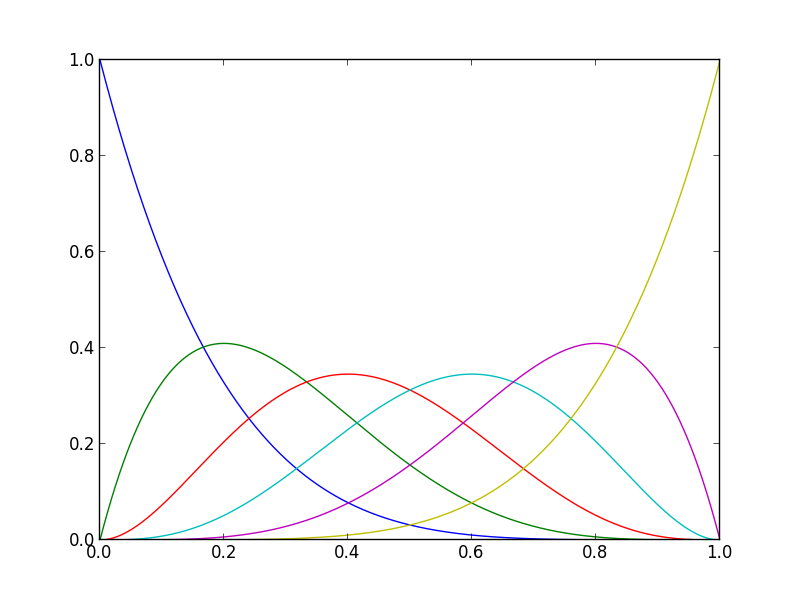
\includegraphics[width=\textwidth]{bernstein_basis}
\caption{5th degree Bernstein basis functions}
\end{figure}

This is a useful property.
B-splines are a generalization of B\'{e}zier curves which allow us to use piecewise basis functions.
Using piecewise basis functions allows us to make local changes to the curve we are representing.
This makes it so that we do not have to recompute the entire curve when we change only one control point.
This also makes control of the curve easier because changes from each contro point are only applied locally.
Another useful effect is that this makes the individual pieces of the B-Spline more responsive to changes in the control points that are used in creating it.
This, again, makes the curve easier to control.
The idea is that each point has a strictly local influence on the curve so that each point has a larger effect on a smaller portion of the curve.

We would like to be able to do this without loosing the useful properties of B\'{e}zier curves.
Simply using basis functions guarantees that each point of the curve will be a linear combination of the control points.
It would be best if we could make it so that this curve has the convex hull property (i.e. that it lies within the area bounded by the outermost control points).
B\'{e}zier curves also allow easy computation of their derivatives, so we would hope that B-Splines would allow this as well.
One of the largest constraints we need is that the curve we are forming be continuous.
It would be even better if it were differentiable, or even twice-differentiable.
The construction of the B-Spline Basis functions takes all of these factors into account.

There are a number of ways the B-Spline basis functions can be defined.
A common approach is to use recursion.
Let $U = \lbrace u_0, u_1, ... , u_m \rbrace$ be a nondecreasing sequence of real numbers.
$U$ is called the knot vector.
The $u_i$ are called the knots.
Note that each $u_i$ is not necessarily distinct.
$N_{i,p}(u)$, the $i$'th B-Spline basis function of degree $p$, or order $p+1$ is defined as:

\begin{equation}
N_{i,0}(u) = 
\begin{cases}
1 & \text{if } u_i \leq u < u_{i+1} \\
0 & \text{otherwise}
\end{cases}
\end{equation}

\begin{equation}
N_{i,p}(u) = \frac{u - u_i}{u_{i+p} - u_i} N_{i,p-1}(u) + \frac{u_{i + p + 1} - u}{u_{i + p + 1} - u_{i + 1}} N_{i+1,p-1}(u)
\end{equation}

This is known as the Cox-De Boor recursion formula.
This algorithm is the De Boor algorithm. 
When implemented properly, this algorithm is both fast and numerically stable.

Notice that we defined $U$ to be nondecreasing, which means some $u_i$ may be repeated.
When programming this algorithm as written, be careful to avoid division by zero.
When we get the indeterminate form $\frac{0}{0}$ we define these terms to be zero.

Also note that $N_{i,0}$ is a step function which is zero except on $[u_i, u_{i+1})$. 
The other basis functions are piecewise polynomials of degree $p$ that are nonzero on $[u_{i-p}, u_{i+1+p})$.
This is also nice because computation of a set of basis functions requires only a knot vector $U$ and a degree $p$, so we can predefine basis functions before we know the actual positions of the control points.

\begin{problem}
Use the De Boor algorithm to write a recursive python function to evaluate a b-spline basis function for some $u$ spanned by the knot vector.
\end{problem}

Upon considering the computation involved in the previous problem, we see that this recursion, particularly for higher order splines, involves a massive amount of repetitive calculation.
Some of this excess computation can be eliminated while still using recursion, but we will do this by forming an iterative solution to the problem.

First, notice that for splines of order $2$ and higher, we actually compute the values of some splines multiple times.
A simple way to avoid this is to figure out which of the 0-order splines we will actually use in our computation, compute them all, then compute all the needed splines of order 1, 2, etc.

There is also some redundant computation in the computation of the coefficients used at each stage of the recursion.
This can be eliminated by using good control structure and a temporary variable.

We will label the left and right coefficients in the formula $L$ and $R$ respectively, so we have $L(n,p,u) = \frac{u - u_i}{u_{i+p} - u_i}$ and $R(n,p,u) = \frac{u_{i + p + 1} - u}{u_{i + p + 1} - u_{i + 1}}$. Notice that $L(n+1,p,u) = 1 - R(n,p,u)$. We can eliminate much of the duplicate computation by computing the new left hand side coefficient the iteration before we actually need it. This avoids nearly all the repeated computation.

\begin{problem}
Write an iterative function that computes the values for all the b-spline basis functions of a given power $p$ for a given array of $u$ values. Return the answer as a two dimensional array.
\end{problem}

It is worth noting that you can remove further excess computation when evaluating a single function and even further when evaluating a single function at a single point.
This can be done by figuring out in advance which of the $N_{i,p}$ will be nonzero and only iterating over those terms.
This approach may or may not be faster depending on the form of the problem.

Scipy has some built in functions and a built in class for B-splines.
They are all part of the scipy.interpolate package.
